\chapter{Tesztelés és mérések}
\label{cha:test}

\section{A teszteléshez használt eszközök}
\label{sec:testtools}

A feldolgozólánc teszteléséhez elő kellett állítani először a komponensek futtatható változatát. A komponensek implementációjakor használt Bndtools eszköz ebben is nagy segítségemre volt, mert az alkalmazás futtatásakor a Bndtools automatikusan előállította a telepíthető csomagokat. Az egyes komponensek könyvtári függőségeit, amelyek nem részei az alap OSGi futtató környezetnek (tipikusan ezek a harmadik féltől származó könyvtárak) magamnak kellett előállítanom szintén a Bndtools segítségével.

A fordításnál előállított JAR formátumú bundle-ök módosítás nélkül telepíthetőek valamilyen OSGi alapú rendszert futtatni képes környezetbe (\textit{bundle repository}-ba). Fejlesztés során a gyorsabb tesztelhetőség miatt az Eclipse saját OSGi implementációs megoldását az Equinox-ot használtam. Egy stabil változat elkészítése után pedig, bizonyos szinten automatizáltan, szkriptek segítségével telepítettem az alkalmazást a SZTAKI Cloud-ban létrehozott virtuális gépre, melyet az alkalmazás futtatására készítettem elő tesztelés céljából.

A telepítési környezetben már a könnyen kezelhető Apache Felix \cite{apachefelix} OSGi implementációját használtam, mert annak WebConsole eszközével könnyedén kezelhetőek a komponensek menedzselése, valamint parancssoros hozzáférés is lehetséges, ahol interaktív módon menedzselhetőek a komponensek, sőt még egy egyszerűbb Bash szintaktikáját utánzó szkriptelési lehetőséget is használhatnak a fejlesztők. Teszteléskor a virtuális gépre SSH-n belépve, az Apache Felix konzolos felületét használva telepítettem az elkészített bundle-öket és függőségeiket.

\begin{figure}[htp]
\centering
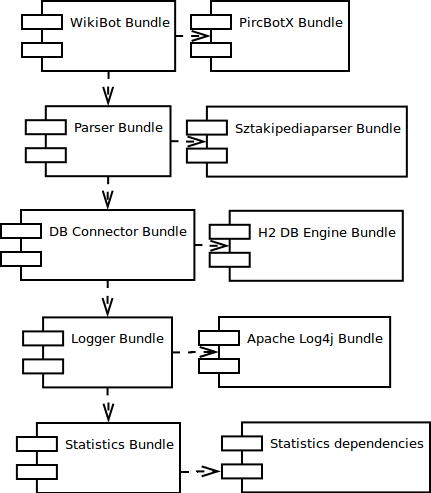
\includegraphics[scale=0.5]{img/deploymentdependency}
\caption{Komponensek függőségei}
\label{fig:deploymentdependency}
\end{figure}

Telepítéshez, illetve a feldolgozólánc komponenseinek frissítéséhez az Apache Felix egy beépített megoldását az Apache Felix Gogo-t használtam, mely egy egységes, szabványos shell felületet határoz meg az OSGi alapú környezetek számára. Amint már említettem az Apache Felix Gogo-val a Unix rendszerekben ismert Bash szintaktikához hasonló parancsokat lehet használni. Ezeket a parancsokat akár szkript formájában is futtathatjuk, ez a Gogo Shell szkript, másnéven \textit{gosh} szkript.

A csomagok függőségeit ábrázolja a \ref{fig:deploymentdependency}.~ábra. A függőségi fa leveleiben található bundle-öket kell először, majd a fában a gyökér felé visszafelé haladva kell a többi bundle-t telepíteni.

A bundle-ök menedzselését a konzolos Apache Felix Gogo Shell-en kívül, egy webes felületen Apache Felix Web Console segítségével is lehet végezni. Segítségével a rendszer állapotát, tulajdonságait lehet beállítani és megfigyelni, valamint a bundle-ök részletes tulajdonságait, kapcsolatait lehet felderíteni, illetve beállításait módosítani. A webes felületről a bundle-ök telepítésével, indításával kapcsolatos funkciók szintén elérhetőek.

% section testtools (end)

\section{A feldolgozóláncra épülő kutatómodul}
\label{sec:researchbundle}

A tesztelés során egy lehetséges felhasználási módot próbáltam ki, mikor a feldolgozólánchoz egy MTA SZTAKI által készített kutatómodult illesztettem. A modul segítségével gépi tanulás, természetes nyelvi feldolgozás témakörökhöz használható program készíthető.

A kutatómodul a feldolgozólánc által készített adatbázisból szerzi meg a bemenő adatokat, ehhez a DB Connector komponens kiegészítése volt szükséges, az OSGi szolgáltatást a lekérdezésekhez szükséges metódussal kellett ellátni.

Az kutatómodul az \textit{WikiZaba} nevet viseli, és az \textit{Annotare} könyvtár képességeit valósítja meg. Célja, hogy XML szabvány szerint jól formázott HTML dokumentumokat nyelvileg feldolgozhatóvá és annotálhatóvá tegyen, így a feldolgozóláncban keletkező Article példányokat fel tudja dolgozni. Az Annotare könyvtárnak három fő funkciója van:

\begin{enumerate}
\item Dokumentum beolvasása SAX Parser segítségével, illetve annak átalakítása. Az átalakítás után keletkezik egyrészt egy plain text dokumentum, amely átadható egy nyelvi feldolgozó modulnak, másrészt egy vagy több lista, amely az XML elemeket, mint annotációkat tartalmazza. 

Az Annotare az \textit{UIMA} terminológiáját használja (de az UIMA kódjait vagy könyvtárait egyáltalán nem, azoktól független). Ebben a terminológiában a szóban forgó plain text dokumentum a \textit{Subject of Annotation} (SOFA), az annotációk pedig \textit{FeatureStructure}-ok reprezentálják. A SOFA alapértelmezett konfigurációban az XML elemek tartalmának konkatenálásából áll össze, de az XML tag-ek elhagyásával. A FeatureStructure-ok egy begin és end pozícióval rendelkeznek, amely pozíció azt jelöli ki, hogy a SOFA-ban hol kezdődik és végződik egy adott annotáció. A feldolgozáskor alapesetben minden FeatureStructure egy XML elemnek felel meg, így a begin és end azt mutatja, hogy hol keződik és hol végződik az adott elem a SOFA stringhez képest. Ez a szám nem azonos azzal a karakterpozícióval, ahol az eredeti dokumentumban az adott XML elem kezdődik, hiszen a SOFA stringbe az XML tag-ek által elfoglalt karakterek nem számítanak bele. 

\begin{lstlisting}[label={lst:annotare}, caption=Példa az XML\, SOFA és FeatureStructure kapcsolatára,breaklines=true]
XML: <a>x<b>y</b><c>z</c></a>
SOFA: xyz
FS-ek: (a) 0..11 ; (b) 4..8; (c) 9..11
\end{lstlisting}

A fentieken túl egyedi konfigurációval megoldható, hogy az Annotare több, közvetlenül egymás után következő pozíciójú, és azonos típusú FeatureStructure-t egybe olvasson.

\item A második fontos funkció a FeatureStructure lista kiegészítése újabb annotációkkal. Ezek rendszerint egy NLP rendszer (például OpenNLP) kimenetéből származnak. Meg kell adni hozzájuk, hogy milyen XML taggel legyen reprezentálva és hogy mi a begin és end koordinátájuk.

\item Végül az Annotare egy FeatureStructure listát képes XML formátumba szerializálni. Mivel a FeatureStructure-ök átlapolódhatnak, nem kell szigorú tartalmazási viszonyban lenniük (szemben az XML elemekkel), ennek a feladatnak fontos része, hogy szükség esetén a rendszer egy FeatureStructure-t több XML elemre daraboljon fel. Azt, hogy melyik elem lesz több részre bontva az elemek prioritása határozza meg, amely egy konfigurálható paraméter a FeatureStructure-ok esetében.
\end{enumerate} 

Az Annotare célja, hogy XML-ként értelmezhető dokumenumokban szereplő szövegeket NLP rendszerekkel feldolgohatóvá tegyen. Tipikusan HTML dokumentumoknál (például a Parsoid parser kimenete) vagy struktúrált dokumentumokat leíró XML fájlok esetén hasznos az alkalmazása. Ezen dokumentumok esetén az a probléma, hogy az XML tag-ek jelenléte teljesen elrontja az NLP rendszerek teljesítményét. Ha ezeket egyszerűen kitöröljük, akkor elveszítünk fontos információkat, ráadásul meg kell oldanunk azt is, hogy az egyik XML elem végén található szó ne olvadjon össze a másik XML elem elején találhatóval. Az Annotare fent részletezett funkciói ebben segítenek. Segítségükkel tetszés szerint vehetünk ki szövegrészeket a dokumentumunkból, feldolgozhatjuk azt, majd az eredményt visszailleszthetjük a strukturált dokumentumunkba.

Az Annotare segítségével tehát a WikiZaba kigyűjti a cikk és kategória hivatkozásokat, majd megállapítja ezek szövegkörnyezetét (azt a bekezdést, amiben szerepelnek), valamint a hivatkozások megjelenési formáját, azaz azt a szövegrészt, amely hivatkozássá alakul. 

% section researchbundle (end)

\section{Mérési eredmények}
\label{sec:measurement}

\begin{figure}[htp]
\centering
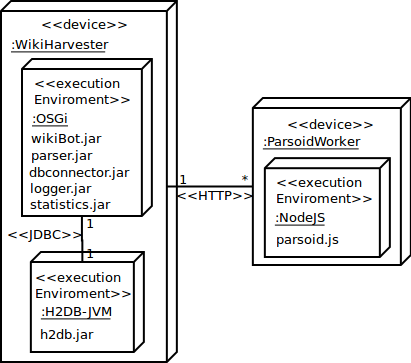
\includegraphics[scale=0.55]{img/deploymentdiagram}
\caption{A mérési összeállítás deployment diagramja}
\label{fig:deploymentdiagram}
\end{figure}

A mérési összeállítás a \ref{fig:deploymentdiagram}.~ábrán figyelhető meg. A használt virtuális gépek OpenNebula sablonjának legfontosabb paraméterei a \ref{lst:opennebulatemplates}.~kódrészletben olvashatóak. A virtuális gépek egy 16 magos AMD 7272 processzorral rendelkező gépen futottak, storage szerverként egy DELL MD3600 rendszer üzemelt. A WikiHarvester gép 4 processzort használ 16 virtuális CPU maggal és 10 Gb RAM érhető el számára. Ezen a gépen fut az OSGi keretrendszer benne a fejlesztett komponensekkel és azok függőségeivel, illetve a H2 adatbázis is itt fut külön folyamatban saját JVM-mel (a H2 adatbázissal JDBC kapcsolaton keresztül történik a kommunikáció). A WikiHarvester gép 30 darab ParsoidWorker virtuális gépet tud használni a cikkek átalakítására a Parser komponensben. A ParsoidWorker gépek 1 darab 2 magos processzort használnak fejenként, 512 Mb RAM memóriával; mindegyikre fel van telepítve a NodeJS, ahol a saját szerveroldali Parsoid megoldás fut.

\begin{lstlisting}[label={lst:opennebulatemplates}, caption=Részlet a használt VM-ek sablonjából,breaklines=true]
NAME   = [APP]WikiHarvester
CPU    = 4
VCPU   = 16
MEMORY = 10240

NAME   = [APP]ParsoidWorker
CPU    = 1
VCPU   = 2
MEMORY = 512
\end{lstlisting}

A mérés megkezdésekor letöltöttem az angol Wikipédiáról egy adatbázis mentést (dump), melynek mérete 42 GB volt. A rendszer indításakor megkezdi a feldolgozólánc a dump feldolgozását egy külön szálon, míg a főszálon on-the-fly követi a Wikipédiába kerülő cikkek változásait. A Wikipédia dump feldolgozása egy előfeldolgozó fázissal kezdődik, ahol a későbbi tényleges feldolgozófolyamat követhetőségéért először meg kell számolni, hogy hány cikket kell beilleszteni a dump-ból. 

\begin{figure}[htp]
\centering
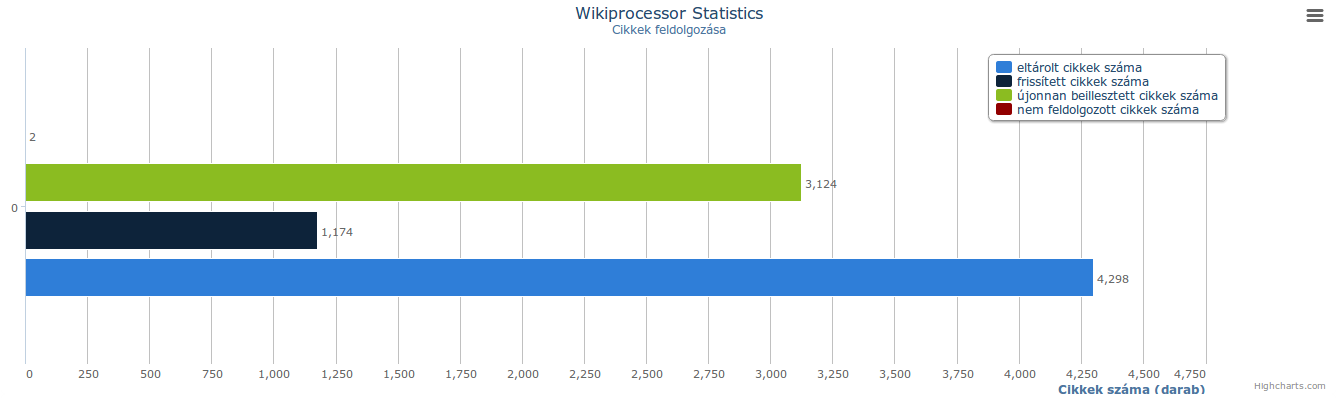
\includegraphics[scale=0.3]{img/storedarticles}
\caption{A mérés során feldolgozott cikkek statisztikája}
\label{fig:storedarticles}
\end{figure}

A fent említett előfeldolgozás a mérés során használt Wikipédia mentéssel körülbelül ~36 percig tartott, ezalatt ~1,36 milliárd cikket olvasott be. Az on-the-fly feldolgozást végző ParsoidWorker-ek száma 25 darab volt, míg a későbbi dump feldolgozást 5 darab ParsoidWorker segítette. Az egy órás mérés végén az adatbázis mérete, üres adatbázissal indítva a mérést 644 Mb lett, ezalatt 4298 cikket dolgozott fel a rendszer. A Statistics komponens által készített részletes feldolgozási statisztikák közül egy látható a \ref{fig:storedarticles}.~ábrán.

\begin{figure}[htb]
\centering
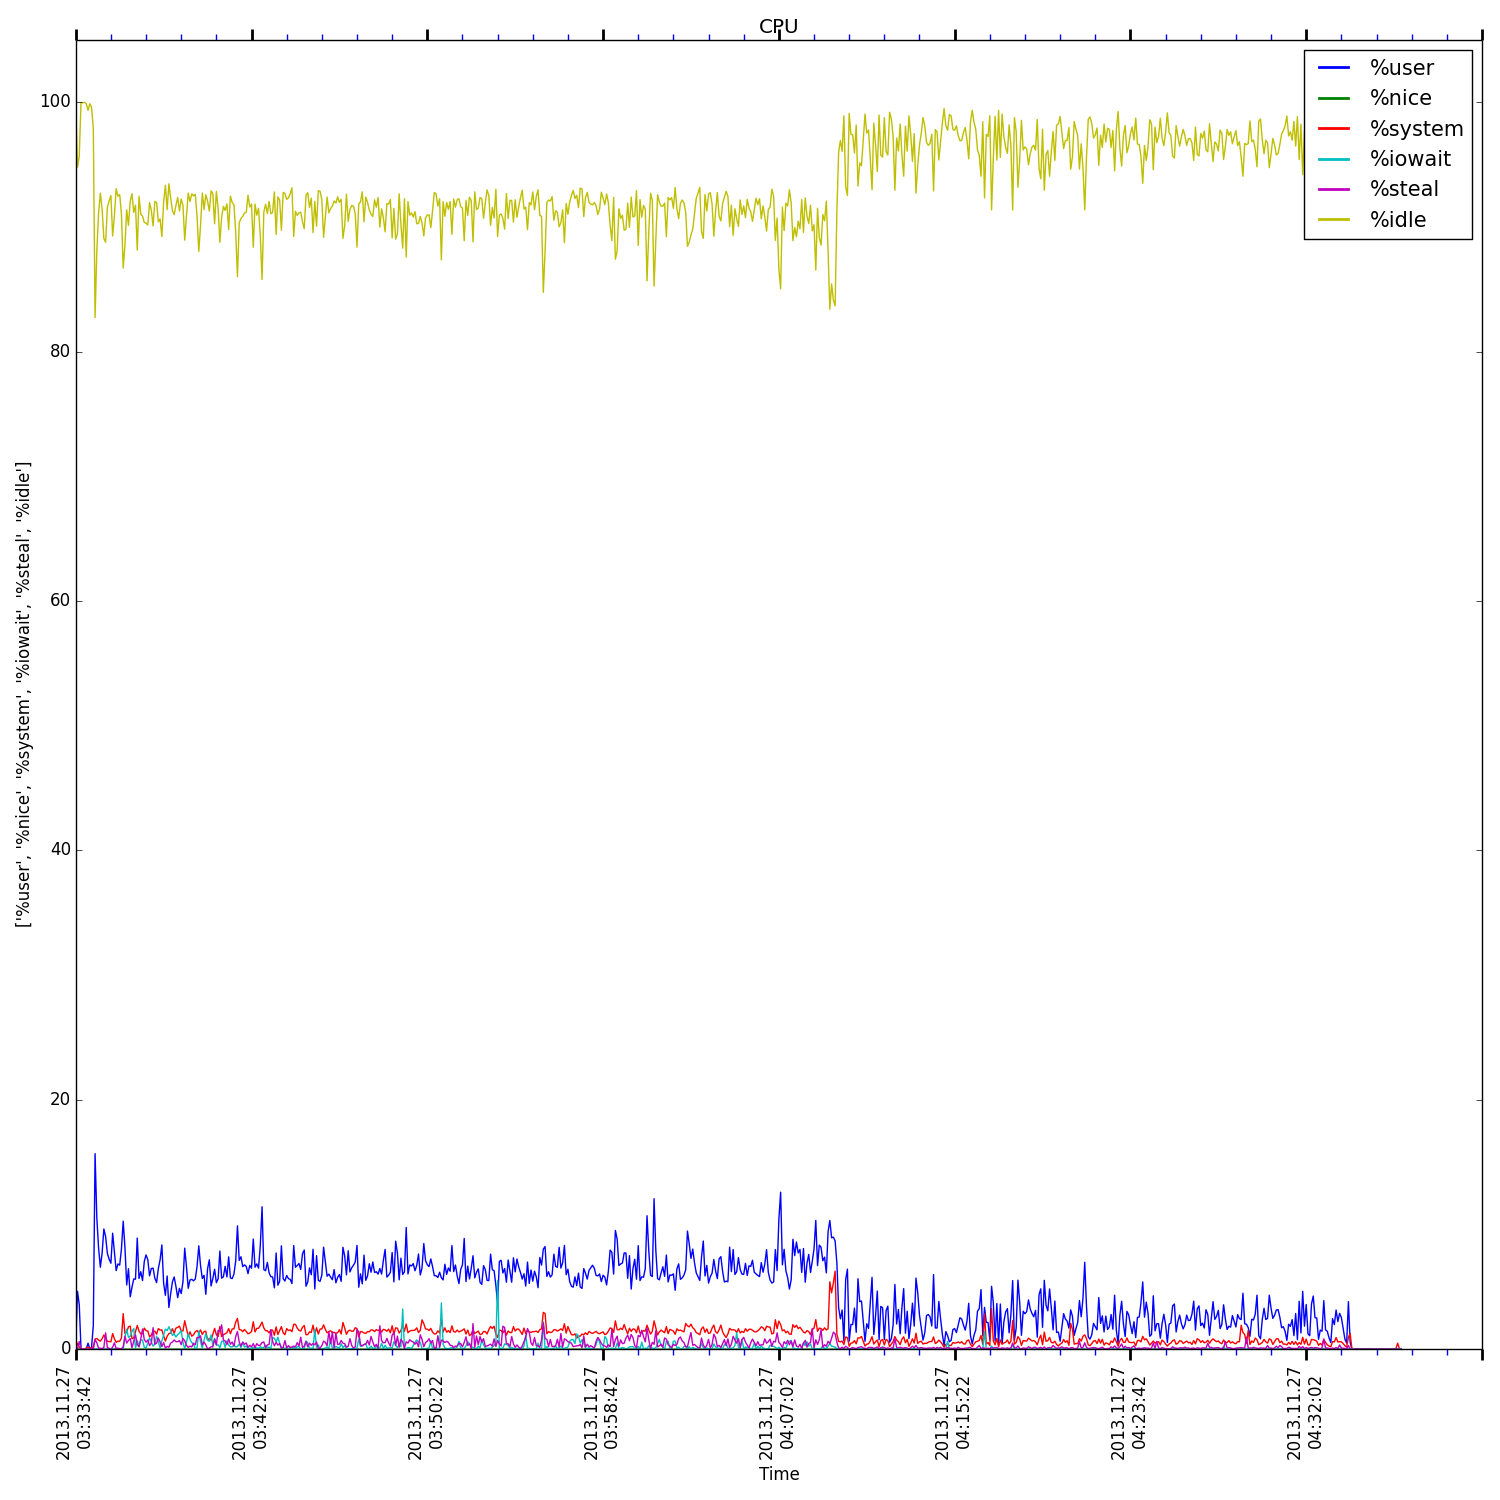
\includegraphics[scale=0.3]{img/measurement_cpu}
\caption{A mérés során mért CPU használat}
\label{fig:measurement_cpu}
\end{figure}

A teljesítményméréseket az \textit{iostat} nevű ingyenes és nyíltforráskódú monitorozó szoftverrel végeztem, mely képes a processzor és a diszk használatot is monitorozni, valamint a különböző szálak működésének megfigyeléséhez a \textit{top} programot használtam. A processzor használatot ábrázoló diagramon (\ref{fig:measurement_cpu}.~ábra) világosan elkülönül az előfeldolgozás fázisa és az a fázis, amikor az on-the-fly és dump feldolgozás egyszerre történik. A mérés eredménye az lett, hogy az alkalmazás által használt processzoridő (\texttt{\%user}, mely a felhasználói módban eltöltött processzoridőt mutatja) körülbelül 2 magot használ ki a rendelkezésre álló erőforrásból, utóbbinál nyilvánvalóan visszaesik kicsit a teljesítmény és átlagosan 1 magnyi erőforrást tud kihasználni a feldolgozólánc.

\begin{figure}[htb]
\centering
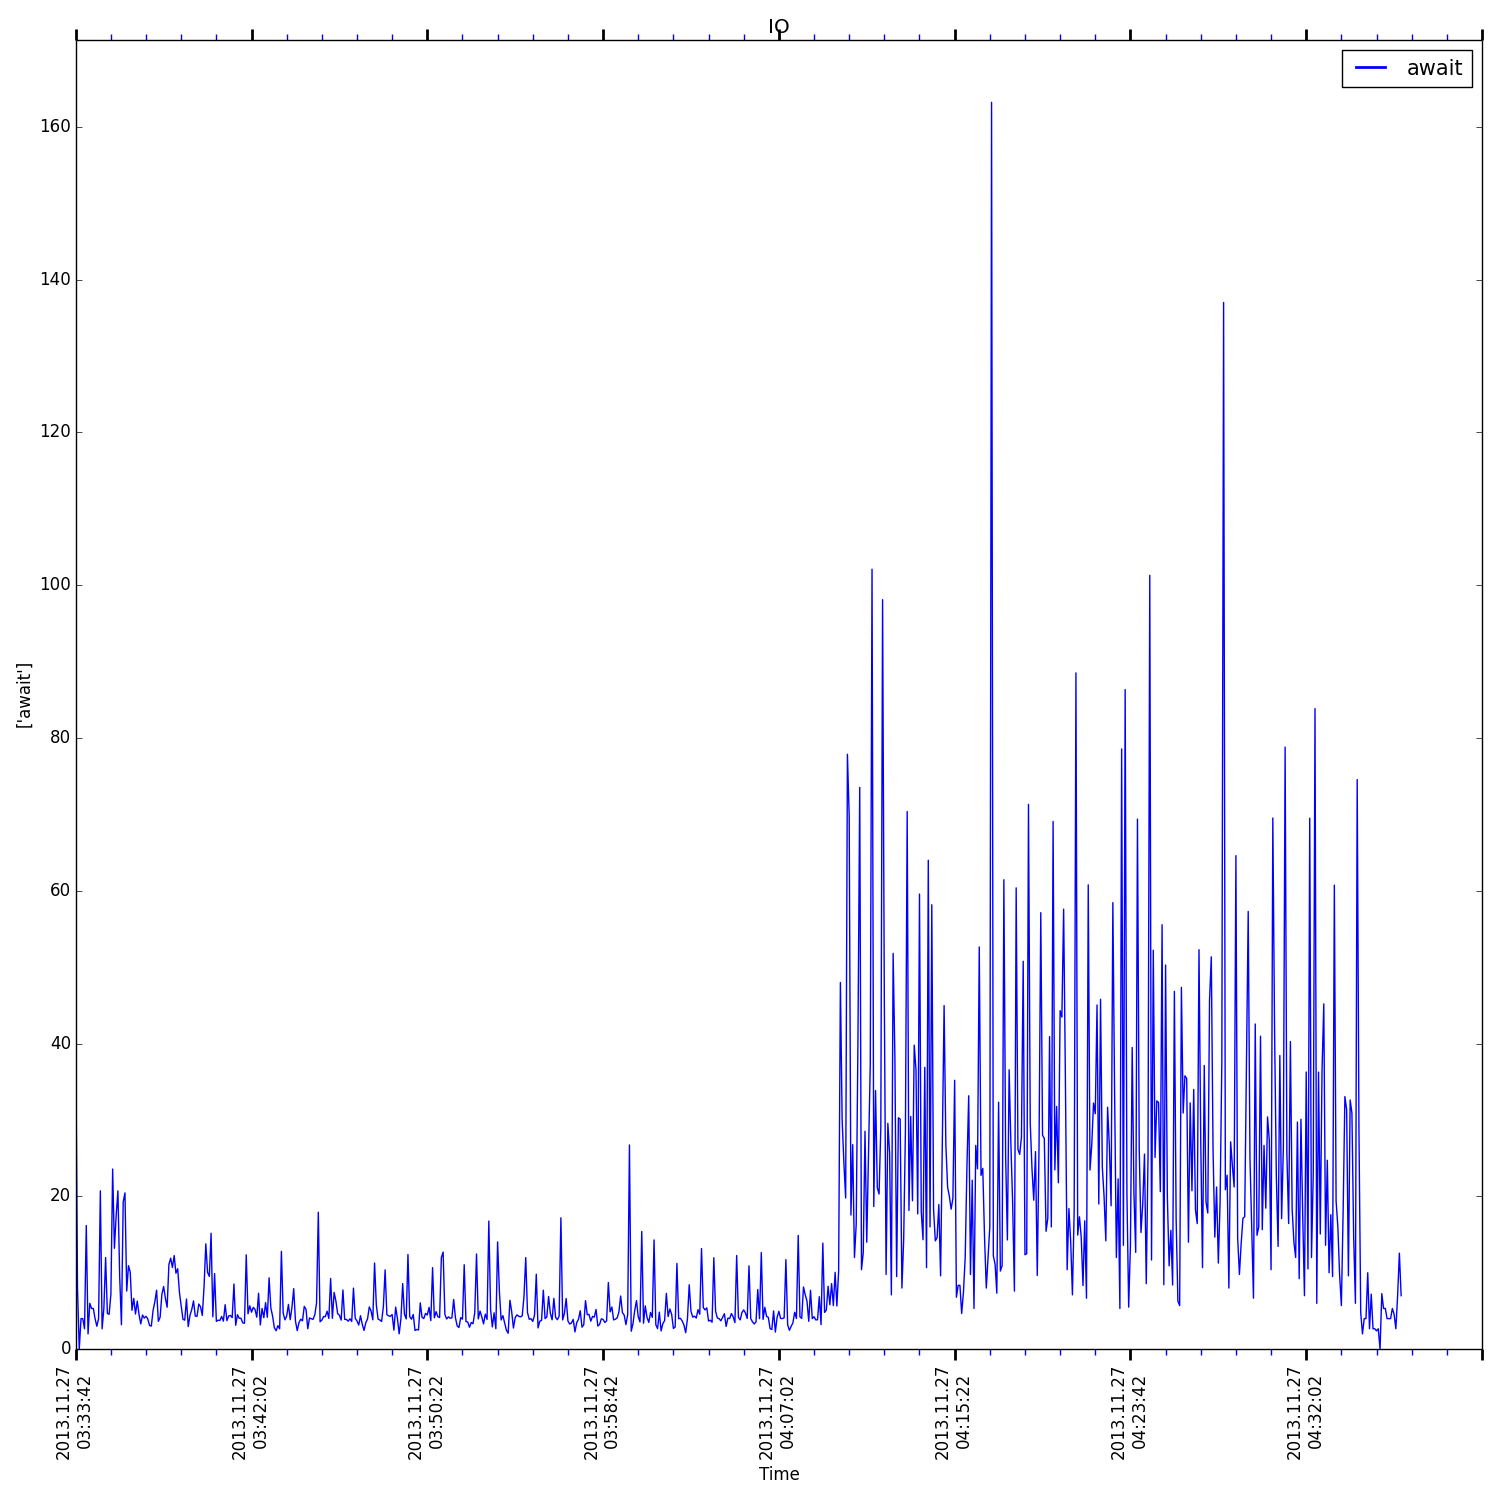
\includegraphics[scale=0.3]{img/measurement_io}
\caption{A mérés során mért lemezhasználat}
\label{fig:measurement_io}
\end{figure}

Kérdés lehet, hogy egy ilyen többszálú alkalmazás, amely több szálat is használ miért nem használja ki a bőséges erőforrást? A válasz az, hogy kihasználja az erőforrásokat, csak a grafikonon ez nem figyelhető közvetlenül meg. Az alkalmazás futásakor a top programban világosan látszott, hogy a feldolgozólánc mind a 16 elérhető magot kihasználta a ThreadPool-oknak köszönhetően, azonban a program futásakor legnagyobb részben a processzor más műveletek elvégzésére vár (ezért ilyen magas az \texttt{\%idle}, azaz tétlenségi idő). Ezen időigényes műveletek hálózati kommunikációt jelentenek: a cikk szövegének letöltése Wikipedia API-n keresztül, kommunikáció a ParsoidWorker-ekkel és várakozás a visszakapott eredményekre. A processzor használat visszaesésére a második részben magyarázat még, hogy a gyorsabb és processzorigényesebb dump feldolgozást végző szálak jobban lefoglalják a processzort a többi szál elől.

Másik kérdés lehet, hogy miért csak ennyi cikket dolgozott fel? A válasz az, hogy egyrészt az on-the-fly érkező cikkek 100\%-a fel lett dolgozva, a dump feldolgozásra állított 5 darab virtuális gép teljesítménye pedig egy teljes dump feldolgozásából ennyit tudott elvégezni a lassú Parsoid használatával 25 perc alatt. Továbbfejlesztési lehetőségekről továbbiakban a \ref{cha:ending}.~fejezetben írok.

A lemezhasználatot bemutató grafikon a rendszer fentiekben meghatározott két állapota még jobban meghatározható, mint a processzorhasználatnál. A lemezhasználati statisztikákból olyan metrikát választottam ki, melyből jó következtetéseket lehet levonni. Ez a metrika az átlagos várakozási idő milliszekundumban, amíg az IO művelet végződik. Látható, hogy az első fázisban viszonylag egyenletesen használja az alkalmazás a diszket, míg a dump feldolgozás fázisában hatalmas kilengések vannak és jobban meghatározza a teljesítményt a hálózati forgalomra való várakozás. Összesítve tehát látható, hogy sem a processzor, sem a diszk teljes erőforrását nem lehet kihasználni a kívánt módon implementált rendszerrel, a hálózati kommunikációra való várakozás miatt; a processzor teljesítménye nem összehasonlítható a hálózati teljesítménnyel.

% section measurement (end)

% chapter test (end)